
\chapter{Práce se systémem}
V této kapitole ukážeme, jak se systém používá jako celek.
Konkrétně ukážeme a popíšeme fotografii STM se zapojeným teplotním sensorem a relé, a dále
screenshot webových stránek.

% STM
\section{STM}

\begin{figure}[tbh!]
\includegraphics[scale=0.11]{../img/prace_se_systemem_stm_kvalitni.jpg}
\caption{Foto STM3210C-Eval board}
\label{stm-foto}
\end{figure}

Na obrázku \ref{stm-foto} vidíme dvě STM zařízení.
To s displejem je STM3210C-Eval board, které používáme v celé práci.
% discovery jako debugger
To druhé je STM32F4-Discovery \cite{STM32F4-Discovery}, které používáme jen kvůli tomu, že je na něm
zabudovaný ST-Link, přes který jednak nahráváme firmware do STM3210C-Eval boardu a jednak ho používáme
pro ladění.
V reálném použití nebude použití STM32F4-Discovery nutné.

% teplotní sensor, relé, joystick, reset button, ...
Do STM3210C-Eval boardu (dále jen STM) je zapojen teplotní senzor Dallas DS18B20 \cite{DS18B20}
a relé.
Konkrétní zapojení do GPIO pinů se dá velice snadno změnit ve zdrojovém kódu.
Dole pod displejem STM je několik tlačítek, joystick a čtyři LED diody.
Z toho reálně využíváme pouze joystick jako vstup a červenou diodu jako notifikaci o tom, že
se v STM stala nějaká chyba.
Černé \uv{reset} tlačítko slouží jako restart firmwaru STM.

Na displeji je aktuálně zobrazen \texttt{MainFrame}.


% Web server
\section{Webový server}

\subsection{Zobrazení všech STM}

\begin{figure}[tbh!]
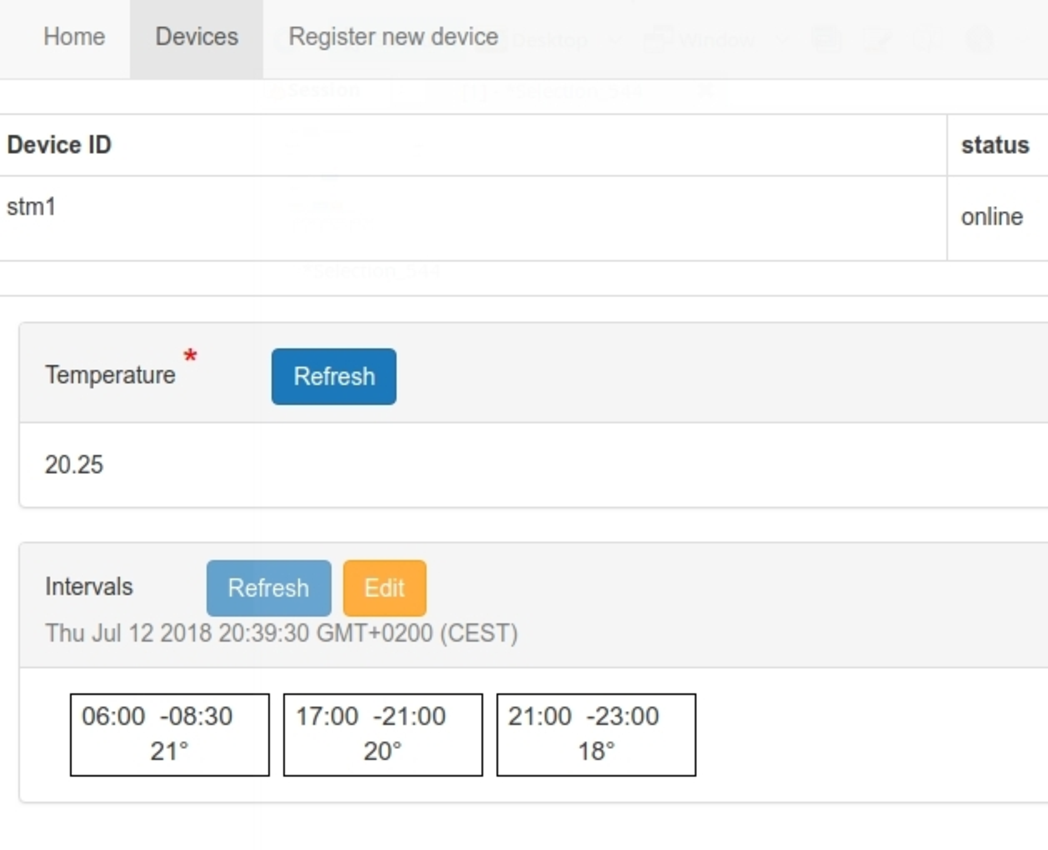
\includegraphics[width=400px, height=400px]{../img/devices_screenshot.pdf}
\caption{Screenshot \uv{devices} stránky}
\label{devices-screenshot}
\end{figure}

Na stránce \ref{devices-screenshot} je vidět jedno zařízení s ID \uv{stm1}, které je zrovna online.
U položky temperature je červená hvězdička, která značí že server přijal od STM novou hodnotu, která
je připravena k aktualizaci pomocí \uv{refresh} tlačítka.
U položky intervals je kromě \uv{reresh} tlačítka vidět i \uv{edit} tlačítko, pomocí kterého můžeme intervaly
libovolně editovat, později uložit a poslat do STM.
Uložení intervalů a jejich následné poslání do STM na screenshotu sice vidět není, nicméně funguje to
tak, že po editaci a uložení intervalů se zobrazí tlačítko \uv{save into device}, pomocí kterého můžeme
intervaly synchronizovat s STM.
U položky intervals je také vidět timestamp.

Dodejme ještě, že takto zobrazených zařízení může na stránce být víc.

% Přidání nového zařízení
\subsection{Přidání nového zařízení}
Přidání nového zařízení je proces, při kterém server vygeneruje nový privátní DES klíč, který uživatel
zadá do STM a to dále šifruje zprávy pomocí tohoto klíče.

Na webový stránkách stačí kliknout na tlačítko \uv{register new device}, zadat ID zařízení a dále
kliknout na \uv{generate new key}.
Server zkontroluje jestli zadané ID je ID existujícího STM a následně vygeneruje DES klíč s omezenou
životností.

